%\usepackage{amssymb}
%\usepackage{amsmath}
\subsubsection{Actividad 1 lab 2}
%*********************
\begin{frame}{}

\pgfdeclareimage[width=\paperwidth,height=\paperheight]{bg}{imagenes/fondo_seccion}
\setbeamertemplate{background}{\pgfuseimage{bg}}

\definecolor{greenU}{RGB}{212,202,72}
\setbeamercolor{block body}{fg=Black,bg=greenU}
\begin{block}{}
	\centering
	\vspace{1mm}
	\large{\textit{Actividades}}
	\vspace{1mm}
\end{block}
\end{frame}
%*********************


%--------------------------------
\begin{frame}{Actvidad 1 lab 2}
\begin{figure}[H]
\begin{flushleft}
Mencione los diferentes tipos de ruido del bloque (noise source), sus características,
describa la función de densidad de probabilidad para cada uno de estos y por que se puede ocasionar
\end{flushleft}
\centering
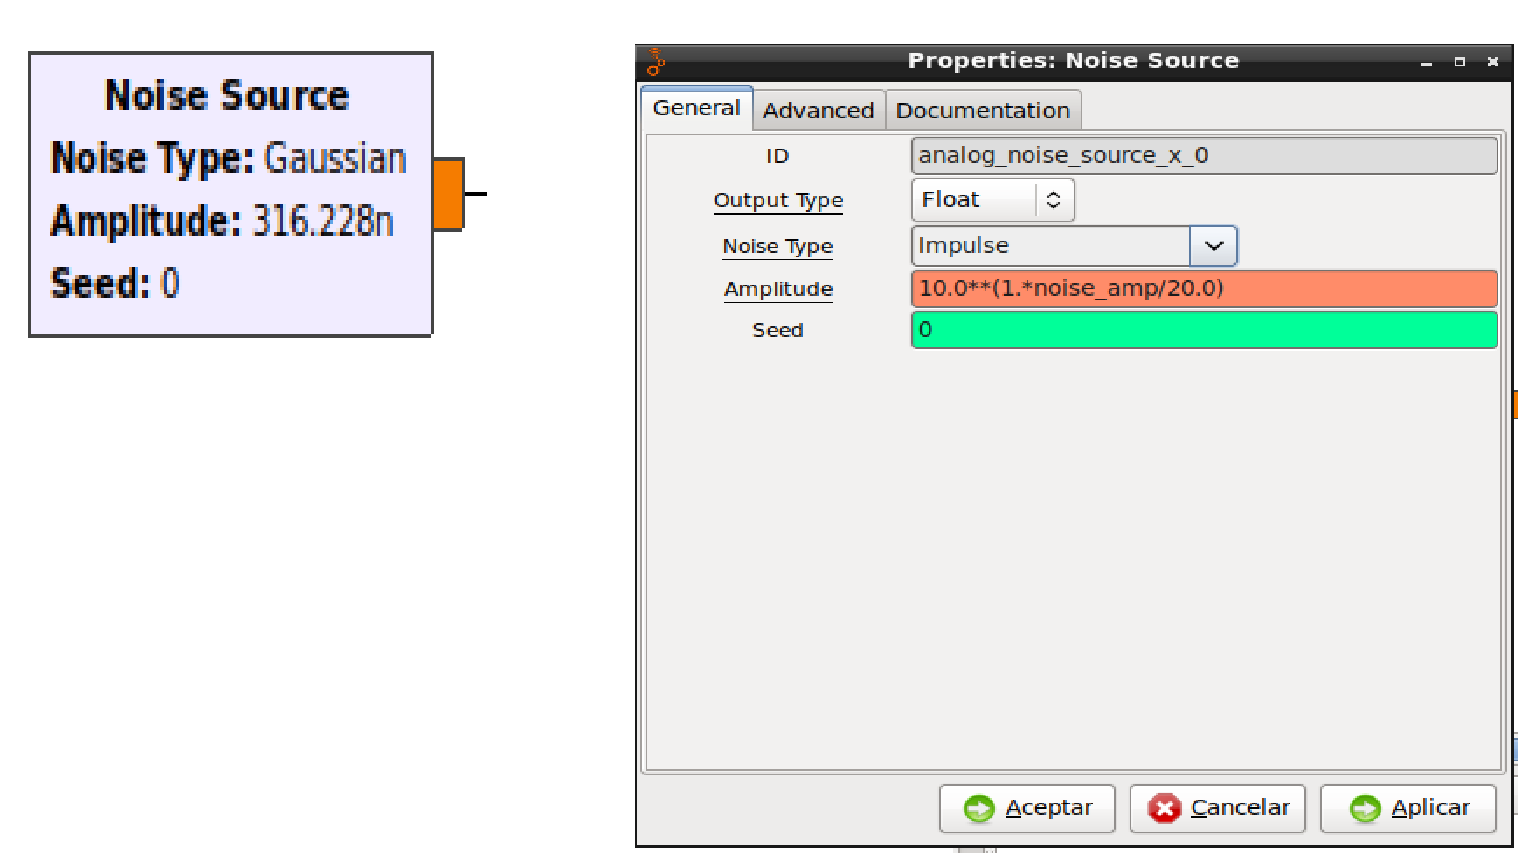
\includegraphics[width=\textwidth, height=0.58\textwidth]{parte1/lab2/pdf/lab2_17.pdf}
\end{figure}
\end{frame}
%--------------------------------

